\section{Módulo de Rastreamento}

	O Módulo de Rastreamento será responsável por rastrear os usuários no ambiente inteligente, determinar a sua localização física em relação ao \textit{Kinect} e gerenciar suas identidades. Para realizar o rastreamento e localização dos usuários é utilizado a biblioteca \textit{OpenNI} (\textit{Open Natural Interaction}). Trata-se de um \textit{framework} que define \textit{APIs} para o desenvolvimento de aplicações de interação natural. Utilizando as imagens de profundidade, a detecção e o rastreamento são feito utilizando subtração de fundo, descrito na Seção~\ref{sec:deteccao-objeto}, e os objetos detectados são representados por suas silhuetas, descrita na Seção~\ref{sec:representacao-objeto}.

	As imagens utilizadas para o rastreamento são imagens de profundidade, exemplificada na Figura~\ref{fig:depthmaps}, providas pelo \textit{Kinect} que são obtidas utilizando o método de Luz Estruturada descrito na Seção~\ref{sec:luz-estruturada}. Tais imagens de profundidade nada mais são que \textit{depth maps} (mapas de profundidade), em que cada pixel da imagem contém o valor estimado da distância em relação ao sensor. O \textit{Kinect} fornece esses dados a uma taxa de $\displaystyle 30 fps$ (\textit{frames} por segundo) com uma resolução $\displaystyle 640px$ x $\displaystyle 480px$.
	

	\begin{figure}[H]
		\begin{center}
			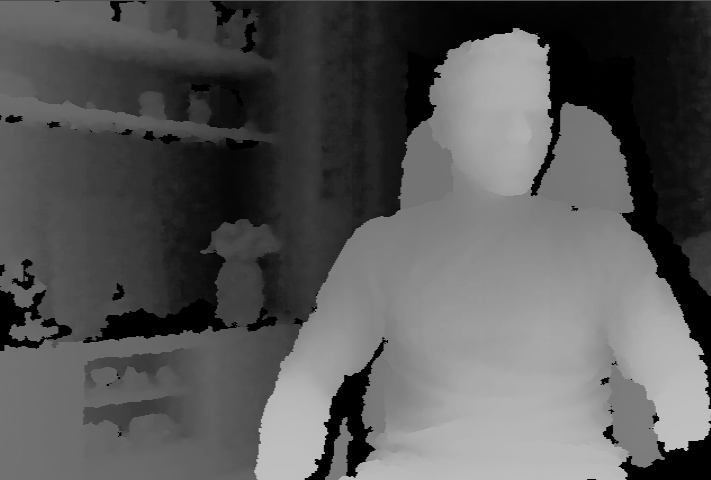
\includegraphics[scale=0.45]{figuras/4.ProblemaEProposta/mapa-profundidade.png}
		\end{center}
		\caption{Exemplo de uma imagem de profundidade fornecida pelo \textit{Kinect}.}
		\label{fig:depthmaps}
	\end{figure}

	Utilizando os mapas de profundidade é possivel calcular as coodernadas $\displaystle (x,y,z)$, em relação ao sensor, de qualquer pixel da imagem. Dessa forma, a posição de um usuário rastreado é determinada utilizando as coordenadas presentes no pixel que representa seu centro geométrico. Sendo assim ao fixar a posição do \textit{Kinect} no ambiente, conseguiremos estimar a localização de qualquer usuário rastreado em tempo real. A Figura~\ref{fig:localizacao} mostra um usuário rastreado pelo Sistema TRUE onde suas coordenadas em relação ao \textit{Kinect} foram estimadas utilizando os valores de profundidade referente ao pixel que representa seu centro de massa geométrico. Os valores das coordenadas $\displaystle (x,y,z)$ estão milimetros.

	\begin{figure}[H]
		\begin{center}
			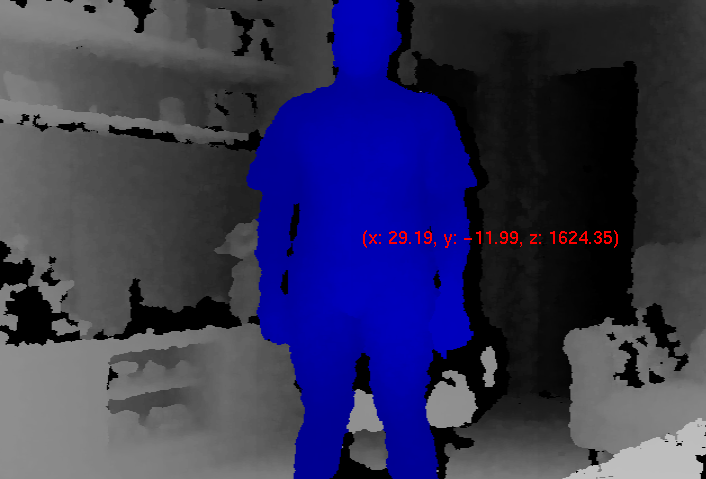
\includegraphics[scale=0.45]{figuras/4.ProblemaEProposta/localizacao.png}
		\end{center}
		\caption{Imagem do Sistema TRUE de um usuário rastreado e localizado.}
		\label{fig:localizacao}
	\end{figure}
	
	
	\begin{figure}[H]
		\begin{center}
			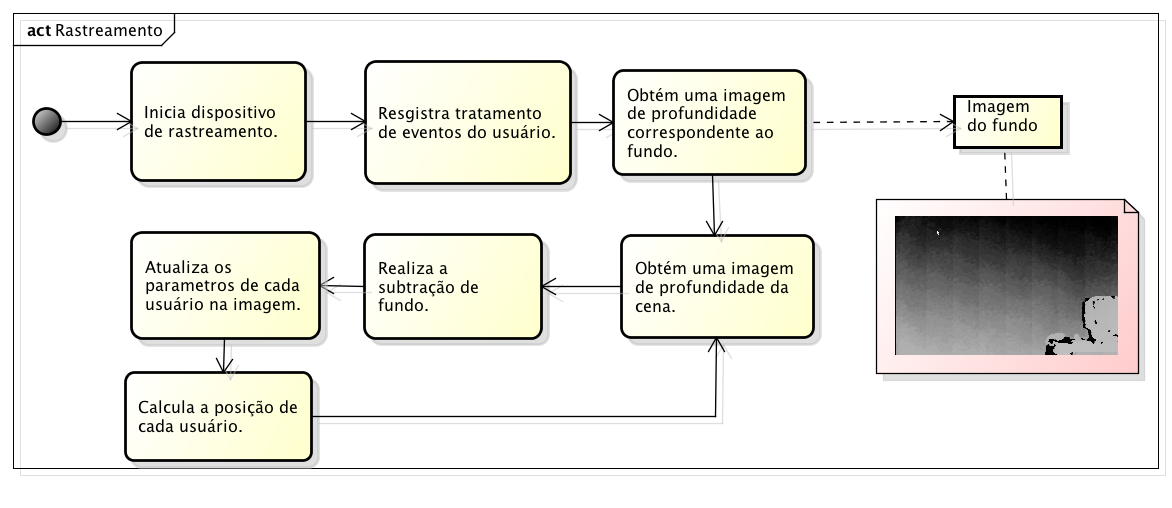
\includegraphics[scale=0.45]{figuras/4.ProblemaEProposta/diagrama-rastreamento.png}
		\end{center}
		\caption{Representação das etapas propostas para o rastreamento.}
		\label{fig:processo-rastreamento}
	\end{figure}
